\section{Simulation Study}
\label{s:simulation}

The design follows the ADEMP structure of \citet{morris2019ademp}. Aims, data-generating
mechanisms, estimands, methods, performance measures and success criteria were written down
before any full run. Departures from that protocol are listed at the end of the design description, before the results.

\subsection{Design}

\subsubsection{Aims}
The study had four aims. The first was to assess the finite-sample bias, standard errors
and coverage of M0 for $(\tau,\kappa,\phi)$ under adoption feedback, adoption related to unit
effects, contagion, overdispersion and small counts (Theorem~\ref{thm:asy}). The second was to
assess inference for cases averted (Theorem~\ref{thm:psi}), and the third to quantify the bias of
the standard estimators and compare it with Theorem~\ref{thm:bias}. The fourth was to assess the
$J$ test and the robustness of M0 when the working model is wrong.

\subsubsection{Data-generating mechanisms}
All scenarios use one generator. Counties are placed
uniformly in the unit square and linked to their six nearest neighbours; the graph is
symmetrised and $W$ is its row-normalised adjacency matrix. Counties are grouped into $G=50$
spatially contiguous strips that play the role of states. Unit effects combine a state
component, a county component and a term proportional to the state's adoption propensity, so
that adoption is related to transmission levels. Outcomes follow the mean \eqref{eq:mean} with
$S=2$ lags, generation-interval weights $(0.85,0.15)$, background input proportional to
population, and negative binomial innovations with shape $k=10$, or Poisson innovations
($k=\infty$). The week-effect level is calibrated so that median county-week counts lie between 5
and 50. Under random adoption, each state's adoption week is uniform on $\{2,\dots,T+2\}$, so
that some states remain untreated within the window. Under feedback adoption, a state adopts
when its lagged incidence first exceeds a threshold that depends on its adoption propensity, and
a county of an adopting state starts when its own lagged incidence exceeds a second threshold.
Adoption is absorbing.

The 25 scenarios form three blocks. The core block crosses $N\in\{500,2000\}$, $T\in\{12,26\}$,
random or feedback adoption, and spillover $(\phi_0,\kappa_0)=(0.4,-0.1)$ or none, $(0,0)$, with
$\tau_0=\log0.8$ (scenarios 1--16). The null block (scenarios 17--20) sets $\tau_0=0$, $N=500$,
$T=12$ with spillover, and crosses the adoption rule with $k\in\{10,\infty\}$. The
misspecification block (scenarios 21--25) uses $N=2000$, $T=26$, feedback adoption and spillover,
and violates one assumption at a time. In X1 the true generation interval is $(0.7,0.3)$ but
$(0.85,0.15)$ is used. In X2 reports are a binomial thinning of infections with a reporting
probability that falls by 15\% after the state adopts. In X3 the effects are unit-specific,
$\tau_i\sim N(\log 0.8,0.1^2)$. In X4 the mean is multiplied by the susceptible fraction, with
cumulative attack rates up to about 20\%. In X5 effects grow with time since adoption from $-0.1$
to $-0.3$.

\subsubsection{Estimands}
The targets are the generating values of $\tau$, $\kappa$ and $\phi$. In
X3 the target of $\tau$ is also compared with the replication-specific mean of $\tau_i$ among
switchers and with the first-order pseudo-true value of Proposition~\ref{prop:hetero}; in X5 the
targets are the event-time effects. For cases averted, the inferential target in each replication
is $\psi^\dagger$, computed from the recursion \eqref{eq:nu} at the true parameter for the treated
unit-weeks and for all unit-weeks after adoption (network). The population quantity $\psi$
of \eqref{eq:psi} is approximated in each scenario from 5000 pairs of policy and no-policy
paths generated with common random numbers.

\subsubsection{Methods}
All methods are applied to the same data sets. The proposed estimator M0 is run together with
its variants M0-G, M0-GI (post hoc), M0-OI, M0-ET and M0$'$ (Section~\ref{ss:computation}).
M1 is Poisson fixed effects with offset $\log\Lambda_{it}(\phi)$ and free $(\kappa,\phi)$
\citep{hausman1984count,wooldridge1999distribution}, and M1-BC is its split-panel jackknife
correction \citep{dhaene2015splitpanel,fernandezval2016individual}. M2 is the two-step log-$R$
difference-in-differences of Theorem~\ref{thm:bias}(a), with weekly reproduction numbers estimated
by the method of \citet{cori2013epiestim}. M3 is two-way fixed effects on $\log(Y+1)$, and M4 is
pooled renewal Poisson quasi-likelihood without unit effects. The infeasible Oracle is Poisson
quasi-likelihood with the true unit effects. All intervals are cluster-robust with $t_{G-1}$
critical values. Failures are recorded per method and are not replaced.

\subsubsection{Performance measures}
For each scenario and method we computed bias, empirical
standard error, mean model standard error and its relative error, and root mean squared error.
We also computed coverage of nominal 95\% intervals, the rejection rates of $H_0\colon\tau=0$ at
the 5\% level and of the $J$ test, and the convergence rate. Each measure is reported with its
Monte Carlo standard error (MCSE). Each scenario used $R=8000$ replications with seeds that depend on the scenario and
replication number.

\subsubsection{Pre-specified criteria}
M0 was to be considered supported if, in the feedback
scenarios, its bias for $\tau$, $\kappa$ and $\phi$ was within 2 MCSE of zero and its coverage
was in $[93\%,97\%]$, while M2 and M3 had biases larger than 2 MCSE or coverage below 90\%. If M1
and M1-BC had negligible bias and correct coverage in every feedback scenario, the contribution
would be limited to the transmission-scale framework, spillover parameters, inference under
contagion and cases averted.

\subsubsection{Departures from the protocol}
The spread of the unit effects was reduced by a factor of 4 to keep counts at $T=26$ within
realistic ranges. M0-G was added before any full run, after a pilot showed multiple roots; M0-GI
was added after interim results and is labelled post hoc wherever it appears. The optional
working-optimal estimator and a group-time average treatment effect estimator were not run.

\subsection{Results}
\label{ss:simresults}

\subsubsection{Contagion present}
Table~\ref{tab:sim-core-tau} and Figure~\ref{fig:core-tau} show
the results for $\tau$ in the core scenarios. In the eight scenarios with spillover, M0 had bias
between $-0.002$ and $0.001$ and coverage between 94.5\% and 95.4\%, under both random and
feedback adoption. Model standard errors matched the empirical standard errors, and their relative
error lay between $-3.5\%$ and $0.9\%$ across $\tau$, $\kappa$ and $\phi$ in all scenarios with
spillover in the core and null blocks (for $\tau$, see Web Table~\ref{tab:sim-m0-full}). Power against
$\tau_0=\log0.8$ was between 77.1\% and 100\%. The spillover parameters were also recovered
(Web Table~\ref{tab:sim-core-spill} and Web Figures~\ref{fig:core-phi} and \ref{fig:core-kappa}).
With $R=8000$, the strict criterion $|\text{bias}|\le2$~MCSE detects very small biases. For
$\tau$ it failed only in scenario 1 (bias $-0.0017$, 2.18 MCSE); for $\kappa$ only in scenario 9
(2.26 MCSE). For $\phi$ it failed in scenarios 1, 2, 3, 9, 10 and 17--20, with the largest bias
0.0035 (5.43 MCSE, scenario 9). Coverage for all three parameters was within the pre-specified
interval. The finite-sample bias of $\hat\phi$ is therefore small but detectable, and the
criterion is met only in a qualified sense. Saying that the bias is small relative to $\phi_0$
holds only when $\phi_0=0.4$: expressed as a fraction of the true value it is at most 0.9\%, but
the absolute bias is the quantity that matters when the true coupling is near zero (next
subsection).

The standard estimators did not meet the criterion. In the spillover scenarios, M1 had bias
between $-0.027$ and $-0.017$ and coverage between 78.1\% and 88.2\%, under random as well as
feedback adoption, as Theorem~\ref{thm:bias}(b) predicts. The split-panel correction M1-BC did
not remove the problem. It converged in only 14.7\% and 23.9\% of replications in scenarios 2
and 4, and its coverage ranged from 25.7\% to 82.7\%. M2 had bias between $-0.110$ and $0.013$,
M3 between $-0.563$ and $-0.030$, and M4 between $0.008$ and $0.139$. Ignoring spillover (M0$'$)
gave bias between $-0.248$ and $-0.114$ and coverage of at most 22.4\%, in line with
Theorem~\ref{thm:bias}(d). The Oracle, which knows the unit effects, had coverage between
91.3\% and 94.8\%. The condition for limiting the contribution was not met.

\subsubsection{Type I error}
Under the null (Web Table~\ref{tab:sim-null} and Web
Figure~\ref{fig:null}), M0 rejected in 4.7\% to 5.2\% of replications, M0-OI in 5.7\% to 6.4\%
and the first event-time bin of M0-ET in 3.9\% to 4.9\%. M1 rejected in 6.3\% to 9.7\%, M1-BC in
14.7\% to 28.6\%, M2 in 76.1\% to 100\% and M3 in 11.9\% to 61.9\%. M4 ranged from 4.6\% to 100\%,
depending on the adoption rule. The $J$ test of M0-OI had size between 4.4\% and 4.9\%.

\subsubsection{No contagion and multiple roots}
When $\phi_0=\kappa_0=0$ the true value lies on the boundary of the parameter space, and this is
the case in which the estimating equations need care rather than the case in which the method has
no answer. Table~\ref{tab:sim-core-tau} and Web Table~\ref{tab:sim-m0gi} report it in the same
format as the rest of the study. A local solver from a fixed start reaches a root of the
just-identified equations that is not the consistent one in about half of the replications; the
bias of $M_0$ for $\tau$ ranged from 0.132 to 0.469 and its coverage from 0.6\% to 38.8\%, the
bias of $\hat\phi$ from 0.232 to 0.888 and that of $\hat\kappa$ from $-0.457$ to $-0.150$.

The root diagnostics identify the mechanism (Figure~\ref{fig:roots} and Web
Table~\ref{tab:sim-roots}). In 47.2\% to 51.7\% of replications the profiled equations had more
than one interior root, and a diagnostic run showed that the spurious root moves with the reference
value $\bar\phi$ of the $\phi$-instrument, which is what makes the profile informative. The $J$
test detects the problem in 6.4\% to 27.2\% of replications, so it complements the profile but does
not replace it.

Two consequences follow for reporting, and both are available from objects the analysis already
produces. First, the profile over $\phi$ separates the single-root case, in which $M_0$ needs no
decision, from the multi-root case, in which the choice must be made explicitly. Second, a global
search over the candidate roots places the estimate on the boundary in 28.6\% to 44.8\% of
replications when selecting with the over-identified criterion of $M_0$-G, and in 63.7\% to 80.9\%
with the criterion of $M_0$-GI, which brings bias down to 0.000 to 0.052 and coverage to 87.5\% to
95.2\%. Because the boundary is the right answer when $\phi_0=0$, a high boundary rate is a
diagnosis rather than a defect. In every scenario with spillover, none of the 8000 replications had
more than one root, so $M_0$, $M_0$-G and $M_0$-GI coincide to all reported digits
(Table~\ref{tab:sim-core-tau}); the rules are used only where the local solver needs them. Web
Appendix~\ref{app:rsel} reports the rules on nine further designs, including $\phi_0$ between zero
and 0.4, which locates where selection on the boundary starts to cost coverage.

In this block $M_0'$, which fixes $\phi=0$, is correctly specified; its bias stayed within
$[-0.000,0.002]$ with coverage of 94.7\% to 95.5\%, which confirms that the moment conditions
identify $\tau$ at the boundary and isolates the multiplicity of roots as the source of the
difficulty. $M_1$ showed biases from $-0.048$ to $-0.008$ with 51.3\% to 91.1\% coverage.

\subsubsection{Misspecification}
Web Table~\ref{tab:sim-misspec} and Web
Figure~\ref{fig:misspec} report the misspecification block. With a wrong generation interval
(X1), the bias of $\hat\tau$ was 0.010 with coverage 94.6\%; the error was absorbed mainly by
$\hat\phi$ (bias 0.516), and the $J$ test rejected in 100\% of replications. When reporting fell
after adoption (X2), $\hat\tau$ had bias $-0.057$ and coverage 59.4\%, $\hat\kappa$ had bias
$-0.294$, and $J$ again rejected in every replication; M1 ($-0.099$) and M2 ($-0.094$) were more
biased. With heterogeneous effects (X3), the bias of $\hat\tau$ was 0.005, both against the
switcher mean and against the first-order value of Proposition~\ref{prop:hetero}, with coverage
94.0\%. Susceptible depletion (X4) left $\hat\tau$ unbiased (bias $-0.000$, coverage 95.2\%).
With dynamic effects (X5), the constant-effect estimator had bias 0.219 relative to
$\tau_0=\log0.8$ and coverage 0\%, so that its mean lay outside the range of the true event-time effects, as
Remark~\ref{rem:dynamic} warns. The $J$ test had no power against this departure (4.7\%), but the
event-time specification M0-ET recovered every event-time effect (bias $-0.000$, coverage 95.3\%
to 95.8\%).

\subsubsection{Cases averted}
Web Table~\ref{tab:sim-psi} reports $\hat\psi$ for the treated
unit-weeks. With spillover, the median relative bias was between $-0.004$ and $0.006$, and
coverage of $\psi^\dagger$ ranged from 85.7\% to 95.4\%; it was below 93\% in scenarios 1, 2, 4
and 10 (92.4\%, 85.7\%, 91.9\% and 90.1\%). The three largest shortfalls occurred with $T=26$,
where the recursion compounds over more weeks. Coverage of the population quantity $\psi$ was lower, between 72.1\% and 92.5\%, as
expected from Remark~\ref{rem:psi}. Without spillover, $\hat\psi$ inherited the bias of M0, with
median relative bias up to 2.474 (scenario 14). Under misspecification the median relative bias
was 3.386 (X1), 1004.524 (X2, coverage 50.8\%), 0.779 (X3) and $-0.994$ (X5, coverage 0\%);
under depletion (X4) coverage of the population $\psi$ fell to 53.5\%. Cases averted are thus far
more sensitive to misspecification than $\tau$.

\begin{figure}[!t]
\centering
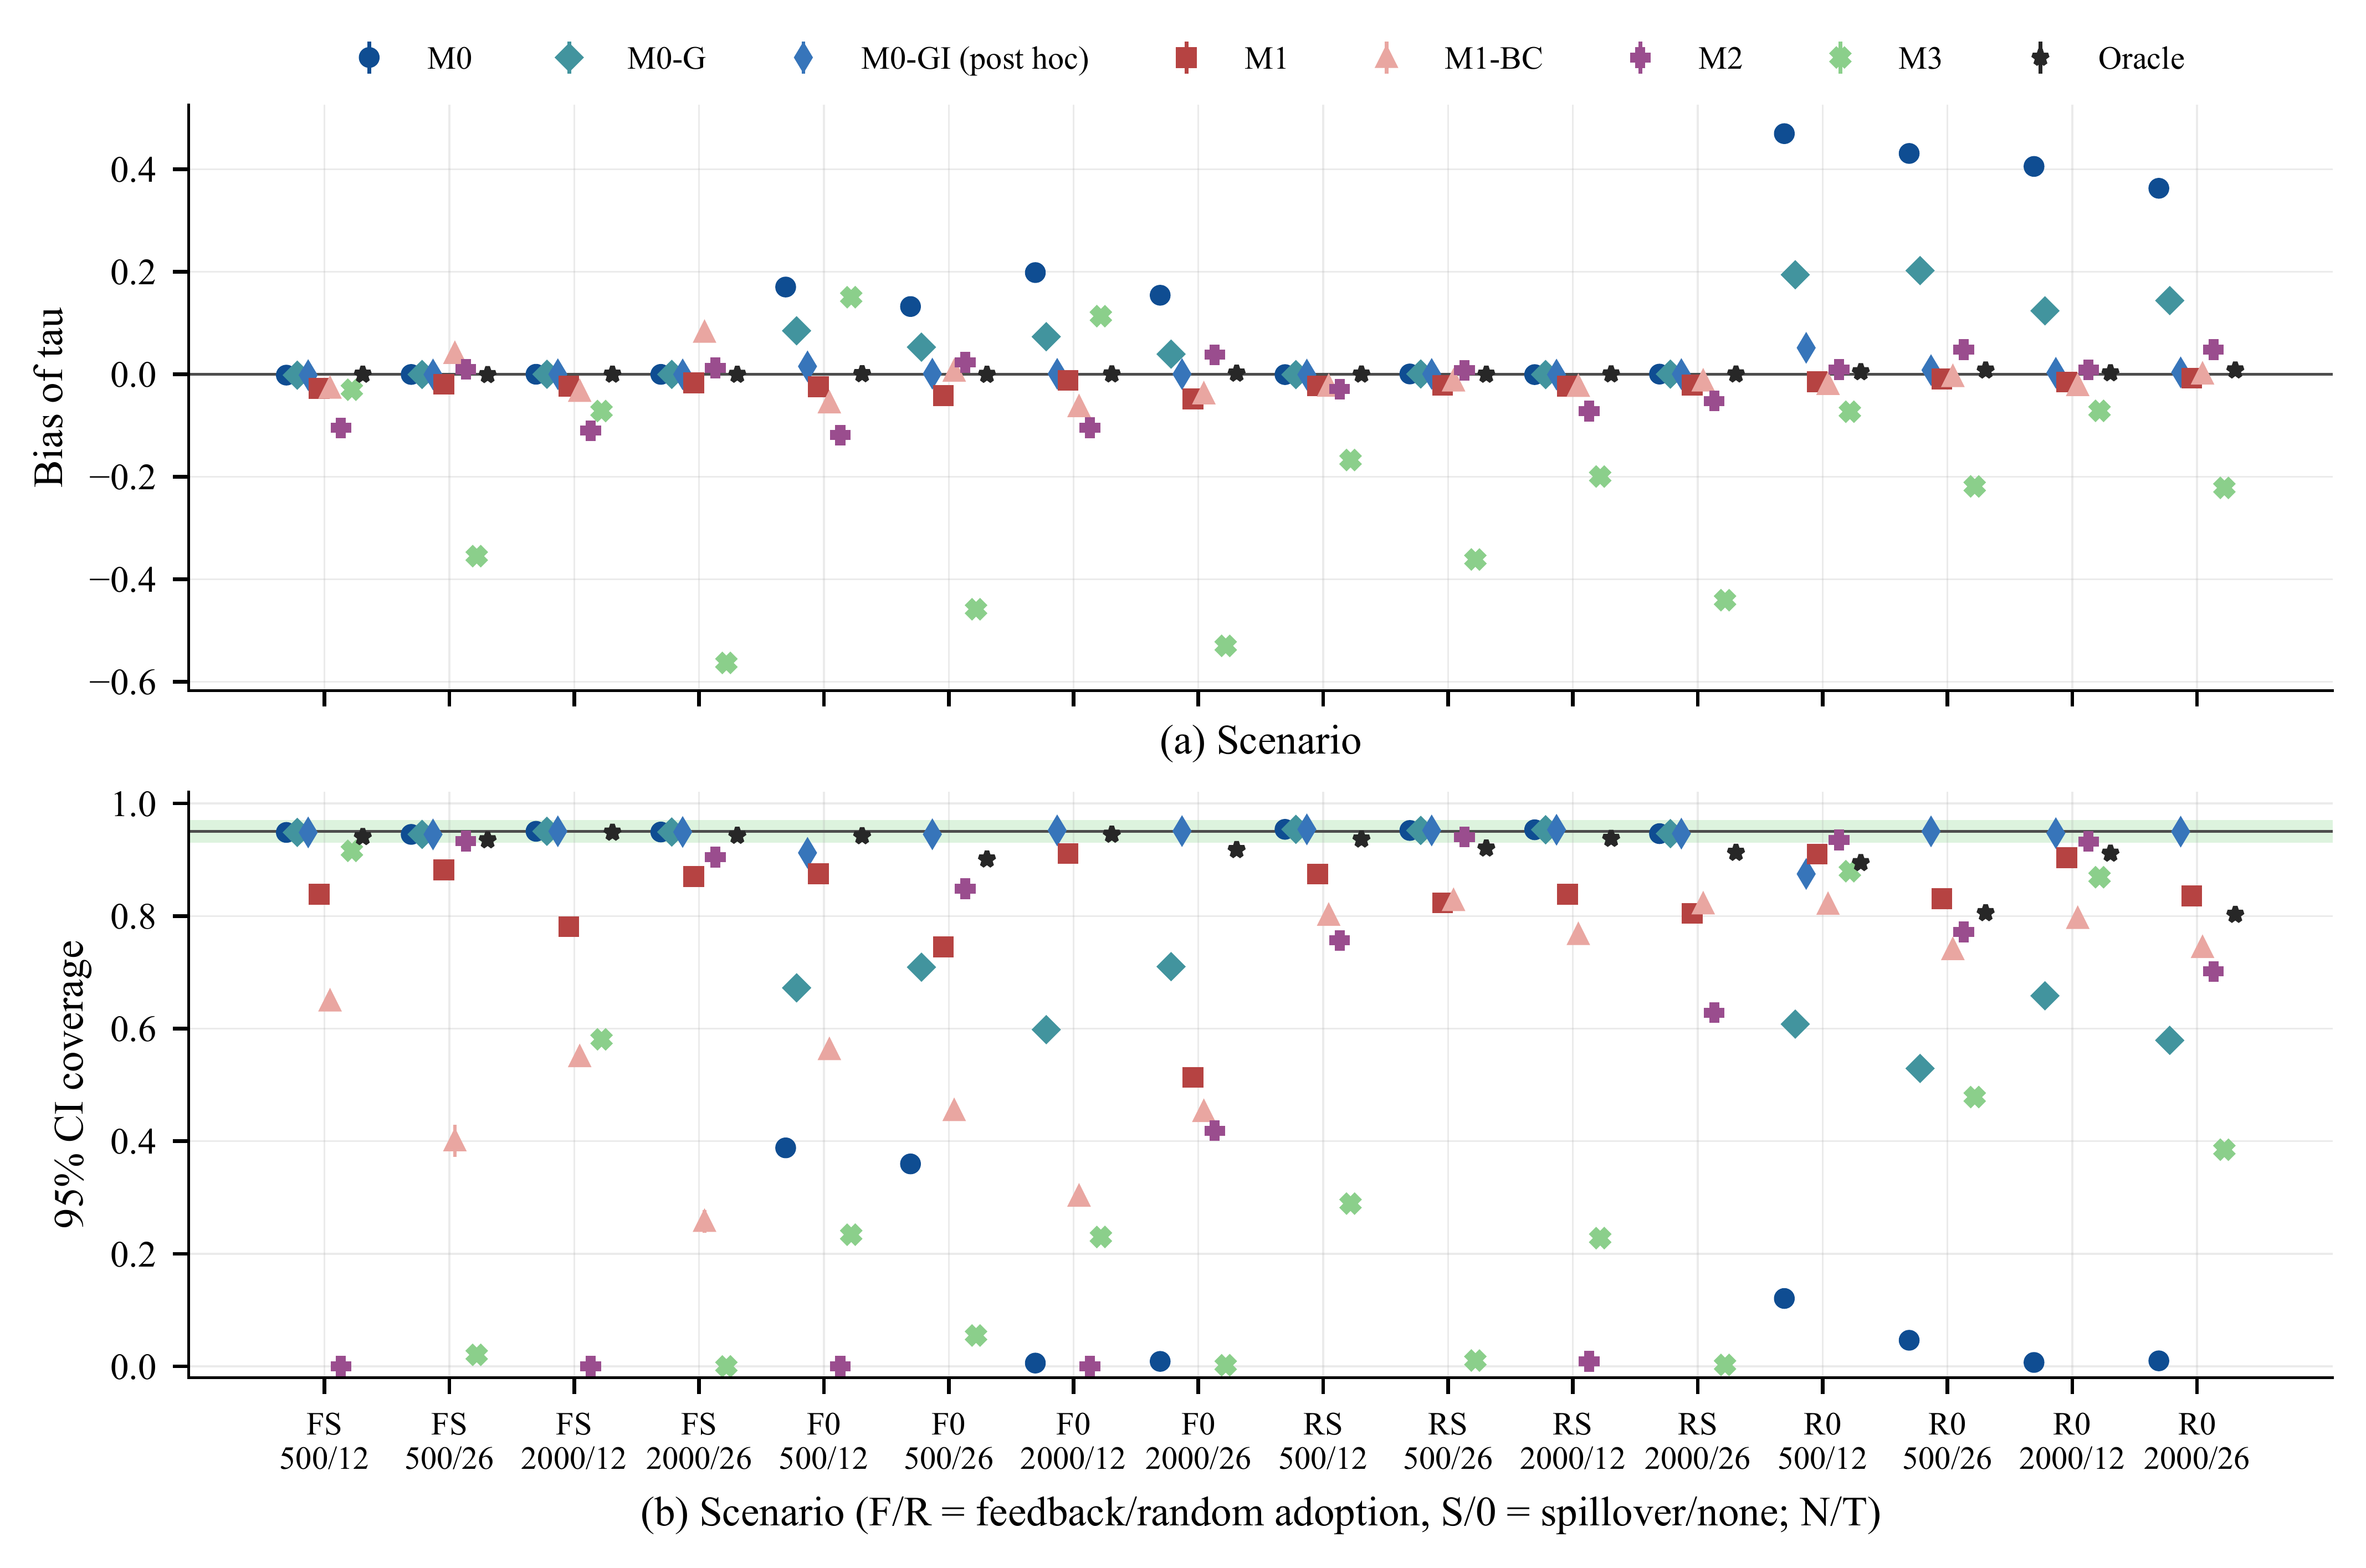
\includegraphics[width=\linewidth]{figures/fig_01_core_tau.png}
\caption{Policy effect $\tau$ in the 16 core scenarios, with (a) bias and (b) coverage of nominal 95\%
$t_{G-1}$ intervals, by scenario and method. Error bars show $\pm2$ Monte Carlo standard errors
and the shaded band marks 93\% to 97\% coverage. $R=8000$ replications per scenario. M0-GI is the
post hoc root-selection variant, evaluated on the same data sets.}
\label{fig:core-tau}
\end{figure}

\begin{table}[!t]
\centering
\caption{Bias (mean of estimate minus true value over replications) and coverage of nominal 95\% confidence intervals for $\tau$ in the 16 core scenarios.}
\label{tab:sim-core-tau}
\footnotesize
\setlength{\tabcolsep}{3.5pt}
\begin{adjustbox}{max width=\linewidth}
\begin{tabular}{ccccrrrrrrrrrrrrrr}
\toprule
$N$ & $T$ & adopt & spill & \multicolumn{2}{c}{M0} & \multicolumn{2}{c}{M0-G} & \multicolumn{2}{c}{M1} & \multicolumn{2}{c}{M1-BC} & \multicolumn{2}{c}{M2} & \multicolumn{2}{c}{M3} & \multicolumn{2}{c}{Oracle} \\
\cmidrule(lr){5-6}\cmidrule(lr){7-8}\cmidrule(lr){9-10}\cmidrule(lr){11-12}\cmidrule(lr){13-14}\cmidrule(lr){15-16}\cmidrule(lr){17-18}
 & & & & bias & cov & bias & cov & bias & cov & bias & cov & bias & cov & bias & cov & bias & cov \\
\midrule
500 & 12 & FB & yes & -0.002 & 94.8 & -0.002 & 94.8 & -0.027 & 83.9 & -0.028 & 64.9 & -0.105 & 0.0 & -0.030 & 91.6 & -0.000 & 94.1 \\
500 & 26 & FB & yes & -0.000 & 94.5 & -0.000 & 94.5 & -0.020 & 88.2 & 0.040 & 40.1 & 0.010 & 93.3 & -0.355 & 2.1 & -0.001 & 93.5 \\
2000 & 12 & FB & yes & 0.000 & 95.0 & 0.000 & 95.0 & -0.023 & 78.1 & -0.034 & 55.0 & -0.110 & 0.0 & -0.072 & 58.1 & -0.000 & 94.8 \\
2000 & 26 & FB & yes & -0.000 & 94.9 & -0.000 & 94.9 & -0.017 & 87.0 & 0.082 & 25.7 & 0.013 & 90.5 & -0.563 & 0.0 & -0.000 & 94.3 \\
500 & 12 & FB & no & 0.170 & 38.8 & 0.085 & 67.2 & -0.024 & 87.5 & -0.056 & 56.2 & -0.119 & 0.0 & 0.150 & 23.4 & 0.001 & 94.2 \\
500 & 26 & FB & no & 0.132 & 36.0 & 0.053 & 70.9 & -0.042 & 74.5 & 0.006 & 45.4 & 0.023 & 84.9 & -0.458 & 5.5 & -0.001 & 90.1 \\
2000 & 12 & FB & no & 0.198 & 0.6 & 0.073 & 59.8 & -0.012 & 91.1 & -0.063 & 30.2 & -0.104 & 0.0 & 0.113 & 23.0 & 0.000 & 94.5 \\
2000 & 26 & FB & no & 0.154 & 0.9 & 0.039 & 71.0 & -0.048 & 51.3 & -0.038 & 45.2 & 0.038 & 41.9 & -0.530 & 0.2 & 0.002 & 91.8 \\
500 & 12 & RD & yes & -0.001 & 95.4 & -0.001 & 95.4 & -0.023 & 87.5 & -0.024 & 80.1 & -0.029 & 75.7 & -0.167 & 28.9 & -0.000 & 93.6 \\
500 & 26 & RD & yes & 0.001 & 95.2 & 0.001 & 95.2 & -0.021 & 82.3 & -0.013 & 82.7 & 0.008 & 94.0 & -0.361 & 1.0 & -0.000 & 92.0 \\
2000 & 12 & RD & yes & -0.001 & 95.3 & -0.001 & 95.3 & -0.023 & 83.9 & -0.024 & 76.7 & -0.072 & 0.9 & -0.199 & 22.8 & 0.000 & 93.8 \\
2000 & 26 & RD & yes & 0.000 & 94.6 & 0.000 & 94.6 & -0.021 & 80.5 & -0.013 & 82.1 & -0.052 & 62.8 & -0.441 & 0.3 & 0.000 & 91.3 \\
500 & 12 & RD & no & 0.469 & 12.1 & 0.194 & 60.8 & -0.014 & 91.0 & -0.020 & 82.0 & 0.009 & 93.5 & -0.073 & 87.9 & 0.005 & 89.4 \\
500 & 26 & RD & no & 0.431 & 4.6 & 0.202 & 52.9 & -0.009 & 83.1 & -0.005 & 74.0 & 0.048 & 77.1 & -0.219 & 47.8 & 0.008 & 80.5 \\
2000 & 12 & RD & no & 0.405 & 0.7 & 0.124 & 65.8 & -0.015 & 90.3 & -0.022 & 79.5 & 0.009 & 93.2 & -0.071 & 86.9 & 0.003 & 91.1 \\
2000 & 26 & RD & no & 0.363 & 1.0 & 0.144 & 57.9 & -0.008 & 83.5 & 0.000 & 74.4 & 0.048 & 70.2 & -0.222 & 38.5 & 0.008 & 80.2 \\
\bottomrule
\end{tabular}
\end{adjustbox}
\par\smallskip\parbox{\linewidth}{\scriptsize Core scenarios, policy effect $\tau_0=\log 0.8$. bias = mean$(\hat\tau)-\tau_0$; cov = coverage (\%) of 95\% $t_{G-1}$ intervals. FB = feedback adoption, RD = random adoption; spill = $(\phi_0,\kappa_0)=(0.4,-0.1)$ vs $(0,0)$. R = 8000 per scenario; largest MCSE: bias 0.004, coverage 1.4 (percentage points). Biases and coverages are computed over converged replications (convergence rates in the supplementary table). M2 and M3 target $\tau$ on different scales and are shown against $\tau_0$ as in the pre-specified protocol.}
\end{table}


\begin{figure}[!t]
\centering
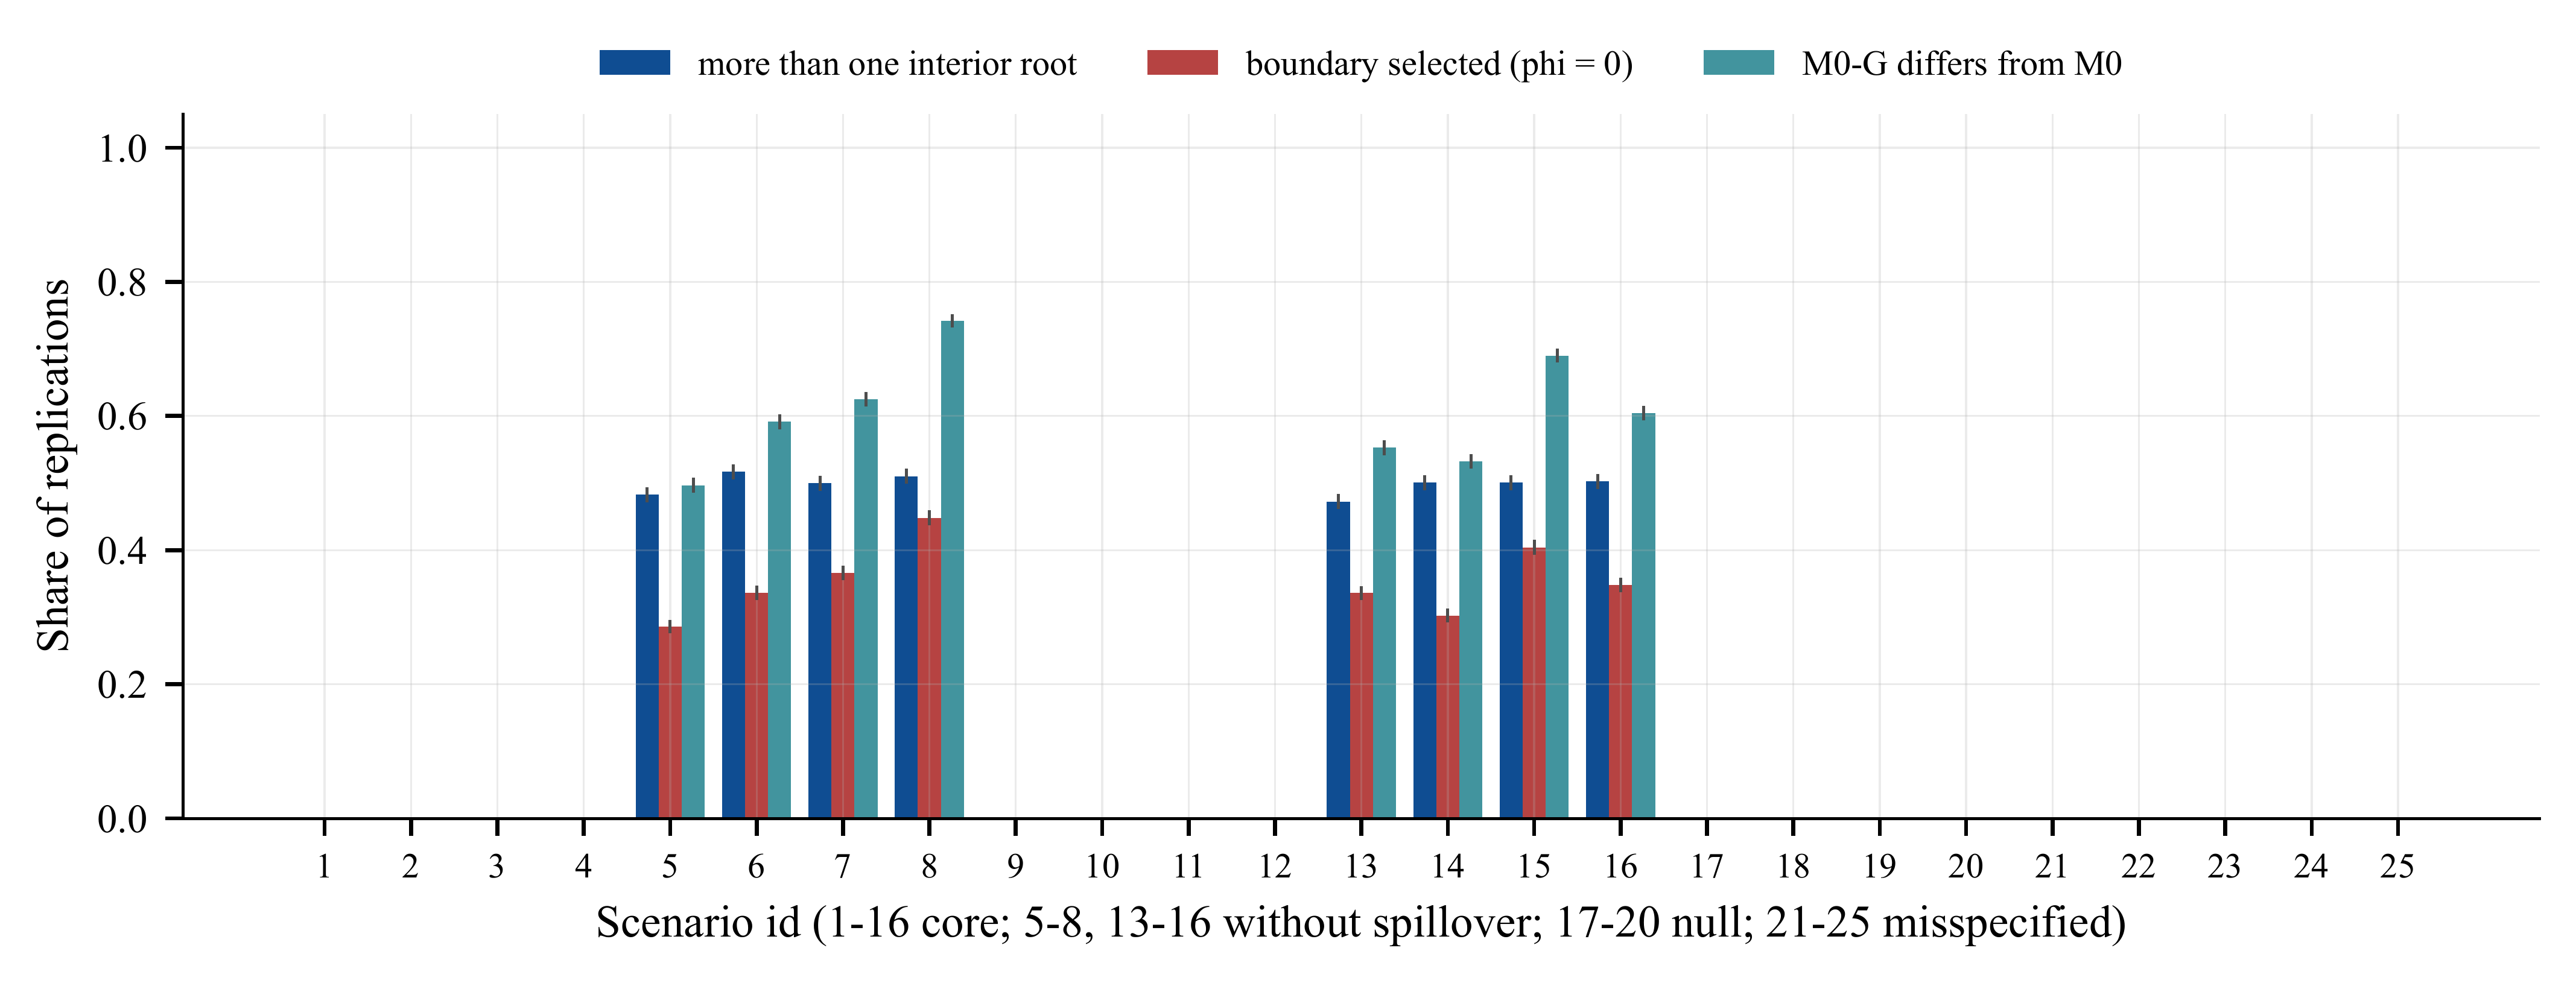
\includegraphics[width=\linewidth]{figures/fig_02_roots.png}
\caption{Root diagnostics of the profiled QD-GMM equations by scenario, from the M0-G grid
search over $\phi\in[0,3]$. Panels show the share of replications with more than one interior root, share in
which the boundary $\phi=0$ is selected, and share in which M0-G differs from M0. Error bars show
$\pm2$ Monte Carlo standard errors. $R=8000$ replications per scenario.}
\label{fig:roots}
\end{figure}

\begin{table}[!t]
\centering
\caption{Post-hoc root selection M0-GI versus the pre-specified M0 and M0-G ($\tau$): bias (mean over replications) and coverage of nominal 95\% confidence intervals.}
\label{tab:sim-m0gi}
\footnotesize
\setlength{\tabcolsep}{3.5pt}
\begin{adjustbox}{max width=\linewidth}
\begin{tabular}{lrrrrrrrrrrrr}
\toprule
scenario & $\phi_0$ & \multicolumn{2}{c}{M0} & \multicolumn{2}{c}{M0-G} & \multicolumn{5}{c}{M0-GI (post hoc)} & boundary & $R_{\rm GI}$ \\
\cmidrule(lr){3-4}\cmidrule(lr){5-6}\cmidrule(lr){7-11}
 & & bias & cov & bias & cov & bias & empSE & modSE & RMSE & cov & GI & \\
\midrule
1 $N=500$, $T=12$, FB, spill & 0.4 & -0.002 & 94.8 & -0.002 & 94.8 & -0.002 & 0.068 & 0.067 & 0.068 & 94.8 & 0.0 & 8000 \\
2 $N=500$, $T=26$, FB, spill & 0.4 & -0.000 & 94.5 & -0.000 & 94.5 & -0.000 & 0.055 & 0.055 & 0.055 & 94.5 & 0.0 & 8000 \\
3 $N=2000$, $T=12$, FB, spill & 0.4 & 0.000 & 95.0 & 0.000 & 95.0 & 0.000 & 0.041 & 0.040 & 0.041 & 95.0 & 0.0 & 8000 \\
4 $N=2000$, $T=26$, FB, spill & 0.4 & -0.000 & 94.9 & -0.000 & 94.9 & -0.000 & 0.037 & 0.037 & 0.037 & 94.9 & 0.0 & 8000 \\
5 $N=500$, $T=12$, FB, no spill & 0.0 & 0.170 & 38.8 & 0.085 & 67.2 & 0.015 & 0.081 & 0.069 & 0.083 & 91.2 & 64.8 & 8000 \\
6 $N=500$, $T=26$, FB, no spill & 0.0 & 0.132 & 36.0 & 0.053 & 70.9 & 0.001 & 0.055 & 0.054 & 0.055 & 94.5 & 78.8 & 8000 \\
7 $N=2000$, $T=12$, FB, no spill & 0.0 & 0.198 & 0.6 & 0.073 & 59.8 & 0.001 & 0.042 & 0.041 & 0.042 & 95.2 & 74.3 & 8000 \\
8 $N=2000$, $T=26$, FB, no spill & 0.0 & 0.154 & 0.9 & 0.039 & 71.0 & 0.000 & 0.036 & 0.036 & 0.036 & 95.1 & 80.9 & 8000 \\
9 $N=500$, $T=12$, RD, spill & 0.4 & -0.001 & 95.4 & -0.001 & 95.4 & -0.001 & 0.082 & 0.081 & 0.082 & 95.4 & 0.0 & 8000 \\
10 $N=500$, $T=26$, RD, spill & 0.4 & 0.001 & 95.2 & 0.001 & 95.2 & 0.001 & 0.070 & 0.069 & 0.070 & 95.2 & 0.0 & 8000 \\
11 $N=2000$, $T=12$, RD, spill & 0.4 & -0.001 & 95.3 & -0.001 & 95.3 & -0.001 & 0.063 & 0.063 & 0.063 & 95.3 & 0.0 & 8000 \\
12 $N=2000$, $T=26$, RD, spill & 0.4 & 0.000 & 94.6 & 0.000 & 94.6 & 0.000 & 0.054 & 0.054 & 0.054 & 94.6 & 0.0 & 8000 \\
13 $N=500$, $T=12$, RD, no spill & 0.0 & 0.469 & 12.1 & 0.194 & 60.8 & 0.052 & 0.178 & 0.102 & 0.185 & 87.5 & 63.7 & 8000 \\
14 $N=500$, $T=26$, RD, no spill & 0.0 & 0.431 & 4.6 & 0.202 & 52.9 & 0.008 & 0.093 & 0.092 & 0.094 & 95.0 & 73.5 & 8000 \\
15 $N=2000$, $T=12$, RD, no spill & 0.0 & 0.405 & 0.7 & 0.124 & 65.8 & 0.003 & 0.075 & 0.071 & 0.075 & 94.7 & 72.8 & 8000 \\
16 $N=2000$, $T=26$, RD, no spill & 0.0 & 0.363 & 1.0 & 0.144 & 57.9 & 0.004 & 0.070 & 0.069 & 0.070 & 95.0 & 75.4 & 8000 \\
17 $N=500$, $T=12$, FB, $k=10$ & 0.4 & -0.001 & 94.9 & -0.001 & 94.9 & -0.001 & 0.055 & 0.055 & 0.055 & 94.9 & 0.0 & 8000 \\
18 $N=500$, $T=12$, FB, $k=\infty$ & 0.4 & -0.000 & 95.2 & -0.000 & 95.2 & -0.000 & 0.029 & 0.029 & 0.029 & 95.2 & 0.0 & 8000 \\
19 $N=500$, $T=12$, RD, $k=10$ & 0.4 & 0.001 & 95.3 & 0.001 & 95.3 & 0.001 & 0.077 & 0.076 & 0.077 & 95.3 & 0.0 & 8000 \\
20 $N=500$, $T=12$, RD, $k=\infty$ & 0.4 & 0.001 & 94.8 & 0.001 & 94.8 & 0.001 & 0.039 & 0.038 & 0.039 & 94.8 & 0.0 & 8000 \\
21 X1: wrong generation interval & 0.4 & 0.010 & 94.6 & 0.010 & 94.6 & 0.010 & 0.036 & 0.036 & 0.037 & 94.6 & 0.0 & 8000 \\
22 X2: reporting drops after adoption & 0.4 & -0.057 & 59.4 & -0.057 & 59.4 & -0.057 & 0.032 & 0.032 & 0.065 & 59.4 & 0.0 & 8000 \\
23 X3: heterogeneous effects & 0.4 & 0.005 & 94.0 & 0.005 & 94.0 & 0.005 & 0.038 & 0.037 & 0.038 & 94.0 & 0.0 & 8000 \\
24 X4: susceptible depletion & 0.4 & -0.000 & 95.2 & -0.000 & 95.2 & -0.000 & 0.037 & 0.037 & 0.037 & 95.2 & 0.0 & 8000 \\
25 X5: dynamic effects & 0.4 & 0.219 & 0.0 & 0.219 & 0.0 & 0.219 & 0.038 & 0.039 & 0.222 & 0.0 & 0.0 & 8000 \\
\bottomrule
\end{tabular}
\end{adjustbox}
\par\smallskip\parbox{\linewidth}{\scriptsize Post-hoc root-selection variant M0-GI (not pre-specified; added after the zero-coupling failure of M0 and M0-G was observed; see the Web Appendix for the protocol record): same candidate roots as M0-G, selection criterion built from the $\phi$-instrument at reference values $0.05$ and $2$ instead of the M0-OI instruments. Same data sets (seeds) as the main run; M0 and M0-G: R = 8000, M0-GI: $R_{\rm GI}$ replications (bias, cov over the replications it reached). boundary. GI = share (\%) of boundary ($\hat\phi=0$) selections. Largest MCSE for M0-GI: bias 0.002, coverage 0.5 (percentage points).}
\end{table}


\subsubsection{Validation on independent designs}
\label{ss:rsel_body}

To check that the rules do not extend beyond the design that
motivated them, nine scenarios with a separate seed base and $R=2000$ replications each were run
over $\phi_0\in\{0,0.05,0.10,0.15\}$, $\bar\phi\in\{0.25,0.5,1\}$ and $G\in\{20,50,100\}$
(Web Table~\ref{tab:rsel}). At $\phi_0=0$ the rule restores coverage (0.888 against 0.361 for
M0). With the coupling small but positive ($\phi_0=0.05$) it costs coverage (0.912 to 0.929
against 0.957 to 0.967) because it selects the boundary in 56\% to 79\% of replications, and at
$\phi_0\ge0.10$ the two rules agree. Global root selection is therefore a remedy when the
profile has several roots, not a default; Web Appendix~\ref{app:rsel} gives the full table.
